% CVPR 2024 Paper Template; see https://github.com/cvpr-org/author-kit
%\usepackage[inkscapelatex=false]{svg}
\documentclass[10pt,twocolumn,letterpaper]{article}


%%%%%%%%% PAPER TYPE  - PLEASE UPDATE FOR FINAL VERSION
% \usepackage{cvpr} % To produce the CAMERA-READY version
\usepackage{cvpr}  % To produce the REVIEW version
% \usepackage[pagenumbers]{cvpr} % To force page numbers, e.g. for an arXiv version

% Import additional packages in the preamble file, before hyperref
%
% --- inline annotations
%
\usepackage[dvipsnames]{xcolor}
\newcommand{\red}[1]{{\color{red}#1}}
\newcommand{\todo}[1]{{\color{red}#1}}
\newcommand{\TODO}[1]{\textbf{\color{red}[TODO: #1]}}
% --- disable by uncommenting  
% \renewcommand{\TODO}[1]{}
% \renewcommand{\todo}[1]{#1}


\usepackage{algorithm}
% \usepackage{algorithmic}
\usepackage{algpseudocode}
\usepackage{amsmath}
% \usepackage{float}
% \usepackage{algorithmicx}


\pagestyle{plain}
\pagenumbering{arabic}

% It is strongly recommended to use hyperref, especially for the review version.
% hyperref with option pagebackref eases the reviewers' job.
% Please disable hyperref *only* if you encounter grave issues, 
% e.g. with the file validation for the camera-ready version.
%
% If you comment hyperref and then uncomment it, you should delete *.aux before re-running LaTeX.
% (Or just hit 'q' on the first LaTeX run, let it finish, and you should be clear).
\definecolor{cvprblue}{rgb}{0.21,0.49,0.74}
\usepackage[pagebackref,breaklinks,colorlinks,citecolor=cvprblue]{hyperref}


%%%%%%%%% PAPER ID  - PLEASE UPDATE
\def\paperID{*****} % *** Enter the Paper ID here
\def\confName{CVPR}
\def\confYear{2024}

%%%%%%%%% TITLE - PLEASE UPDATE
\title{Assignment 3: Cryptocurrency Trend Predictions\\
a Case Study of Different Sequence models on Ethereum(ETH) \\
by Hyperparameter Tuning and Model Complexity}  % **** Enter the paper title here

%%%%%%%%% AUTHORS - PLEASE UPDATE
\author{Zhengyang li\\
   School of Computer and Mathematical Sciences\\
   Adelaide, South Australia 5005 Australia\\
   \tt\small Zhengyang.li01@adelaide.edu.au}
% For a paper whose authors are all at the same institution,
% omit the following lines up until the closing ``}''.
% Additional authors and addresses can be added with ``\and'',
% just like the second author.
% To save space, use either the email address or home page, not both

\begin{document}
\maketitle
\begin{abstract}
   Here in this paper, the application of Recurrent Neural Networks (RNNs) and Long Short-Term Memory (LSTM) models are investigated for predicting financial market trends using a decade's worth of daily data. Our findings reveal significant limitations of these models in handling extended time-series, particularly reflected in decreased accuracy with longer datasets. The study highlights the challenges in capturing long-term dependencies and adapting to the complex, non-stationary nature of financial markets. We also emphasize the importance of feature selection and the integration of traditional financial analysis techniques to enhance model performance. Furthermore, our results suggest that simpler models might be more effective in noisy environments like stock markets, advocating for a nuanced approach in model complexity and an exploration of online learning strategies for real-time market adaptation. This research contributes to a better understanding of the application and limitations of deep learning in financial time-series analysis. Note that all the code and dataset can be found on the: \href{https://github.com/David-Lzy/Deep_Learning_Fundamentals}{Github}
\end{abstract}

\section{Introduction}

Virtual currencies have emerged as a groundbreaking phenomenon in the realm of global finance, reshaping traditional notions of money and the exchange of value. Among the myriad of cryptocurrencies that have proliferated over the past decade, Ethereum (ETH) stands out as a pioneering platform that extends beyond the realm of mere digital currency~\cite{cryptocurrencyJFEC, cryptocurrencyCybersecurity}. Its inception in 2015 marked a significant milestone in the world of blockchain technology, introducing the revolutionary concept of "smart contracts" and enabling a new era of decentralized applications (dApps). To comprehend the evolution of Ethereum and its profound impact on the financial landscape, it is imperative to delve into the comprehensive history of virtual currencies.

The journey of virtual currencies began with the launch of Bitcoin in 2009 by the enigmatic pseudonymous figure known as Satoshi Nakamoto. Often hailed as digital gold, Bitcoin introduced the concept of a decentralized, peer-to-peer digital currency operating on a blockchain – a distributed ledger technology. Bitcoin's primary function was to serve as a medium of exchange and store of value, enabling users to conduct transactions without reliance on intermediaries such as banks or payment processors. Its monumental success catalyzed the creation of numerous alternative cryptocurrencies, collectively known as altcoins, each striving to refine Bitcoin's design or offer distinctive features.

While Bitcoin laid the foundation for the cryptocurrency revolution, Ethereum expanded the realm of possibilities by introducing the concept of smart contracts. Launched in July 2015 by the visionary young programmer Vitalik Buterin, Ethereum was conceived as a blockchain platform capable of facilitating not only digital currency transactions but also the execution of self-executing, programmable contracts. Smart contracts are computer programs that automatically execute predefined actions when specific conditions are met, obviating the necessity for intermediaries in a multitude of contractual agreements. This groundbreaking innovation flung open the doors to a wide array of decentralized applications capable of autonomous and transparent operation, giving rise to the concepts of decentralized finance (DeFi), non-fungible tokens (NFTs), and more.

Traditionally, quantitative trading strategies were primarily rooted in conventional machine learning techniques~\cite{Szegedy15}. These methods involved utilizing algorithms to scrutinize historical market data, recognize patterns, and formulate predictions. Features such as moving averages, relative strength indices, and simple regression models were commonly employed to inform trading decisions. While these approaches achieved some level of success, they grappled with limitations in capturing the intricate and dynamic relationships inherent in financial time series data.

The advent of deep learning marked a transformative shift in the field of quantitative trading. Deep learning techniques, particularly neural networks, heralded the potential to model intricate patterns and dependencies within financial data. Neural networks consist of layers of interconnected neurons, each processing and transmitting information to the subsequent layer. This architectural design excelled at capturing nonlinear relationships, a critical advantage in financial markets where patterns often exhibit intricacies and nonlinearity~\cite{Szegedy15}.

Within the domain of deep learning, recurrent neural networks (RNNs) and their variant, long short-term memory (LSTM) networks, have emerged as indispensable tools for time series analysis~\cite{FuzzyInferenceLSTM}. RNNs are specifically engineered to handle sequences of data, rendering them particularly well-suited for the analysis of time series data. What sets LSTMs apart is their unique ability to capture long-range dependencies within sequences, a challenge that traditional RNNs grapple with due to the vanishing gradient problem. LSTMs employ a memory cell that can retain and update information over extended time intervals, empowering them to recall and leverage past information when making predictions about future data points. In the context of quantitative trading, LSTMs prove invaluable for learning complex temporal patterns, thereby enhancing their utility in predicting price movements, identifying trading signals, and managing risk.

However, the virtual currency market differs significantly from traditional stock markets in several ways. The virtual currency market operates around the clock, unrestricted by geographical locations or market exchanges, leading to greater volatility and price fluctuations. Additionally, the virtual currency market is relatively young and influenced by different factors, such as social media, news events, and regulatory changes, which sets it apart from traditional stock markets. The liquidity in the virtual currency market can experience substantial fluctuations, with some smaller-cap cryptocurrencies susceptible to manipulation. This presents additional challenges in executing trading strategies and managing risks. Compared to traditional stock markets, virtual currency markets may exhibit more non-stationarity in terms of price and trading volume, implying that time-series data may display more trends, seasonality, and periodicity, necessitating additional preprocessing steps to address these non-stationarities. Price volatility in the virtual currency market can be highly pronounced, often accompanied by noise, potentially leading models to produce misleading signals in the short term, thus requiring effective filtering and noise handling strategies.

By integrating LSTMs into the quantitative trading framework, we can harness their capabilities to analyze historical market data and make well-informed trading decisions. Their aptitude for modeling intricate time series patterns can confer a competitive edge in the dynamic and rapidly evolving landscape of virtual currency trading. In this project, we will explore the efficacy of LSTMs in predicting the price of Ethereum, a leading cryptocurrency that has witnessed a meteoric rise in popularity and adoption over the past few years. We will train series od RNN and LSTM models on historical Ethereum price data and evaluate its performance in predicting future price movements. We will also explore the impact of hyperparameter tuning on the models' performance and examine the efficacy of the models in generating trading signals.


In this paper, we delve into the intricacies of applying advanced time-series models to the domain of financial market prediction. Following the introduction, we begin our exploration in Section \ref{sec:method}, where we outline the methods employed, starting with Feature Engineering. This section provides a detailed examination of various technical indicators such as the Relative Strength Index (RSI), Bollinger Bands, Moving Averages, Moving Average Convergence Divergence (MACD), Average True Range (ATR), and On-Balance Volume (OBV). We then discuss the core Time Series Models used in our study, specifically focusing on Recurrent Neural Networks (RNNs) and Long Short-Term Memory (LSTM) Networks. Section \ref{sec:experimentation} is dedicated to the Experimentation process, beginning with Data Preprocessing which includes Data Acquisition and Data Augmentation and Price Normalization techniques. It further elaborates on the Experimentation Environment, detailing the computational setup, and concludes with a thorough discourse on Experimental Parameters and Model Hyperparameter Selection. In Section \ref{sec:results}, we present our Results, highlighting the Challenges Posed by Extended Time-Series in Training and exploring the Limitations of RNN and LSTM models in this context. Finally, in Section \ref{sec:summary}, we provide a comprehensive Summary and Conclusion of our findings. This section synthesizes the insights gained from our experiments and discussions, offering a critical perspective on the efficacy of deep learning models in financial time series forecasting and suggesting potential avenues for future research.

\section{Method} \label{sec:method}
\subsection{Feature Engineering}

In the realm of time series forecasting, particularly in the context of quantitative trading strategies for cryptocurrencies, it is suboptimal to rely solely on raw price data as the primary input for predictive models. The inherent volatility and noise within cryptocurrency price movements make raw prices a less reliable predictor, potentially leading to overfitting and poor generalization in unseen market conditions. To mitigate these risks, it is imperative to employ a more sophisticated approach to feature engineering. This involves transforming raw price data using traditional financial analysis techniques such as the Relative Strength Index (RSI), Bollinger Bands, Moving Average Convergence Divergence (MACD), Average True Range (ATR), and On-Balance Volume (OBV). These methods provide a more nuanced understanding of market dynamics by highlighting trends, volatility, and trading momentum, thereby enriching the input dataset for the AI models. In summary, the integration of these traditional financial analysis tools into the preprocessing stage forms a crucial part of developing a robust and effective cryptocurrency trading strategy using AI.

\subsubsection{Relative Strength Index (RSI)}

The Relative Strength Index (RSI) is a widely used momentum oscillator in the field of technical analysis. It was developed by J. Welles Wilder and is employed to assess the speed and change of price movements. RSI oscillates between 0 and 100 and is typically utilized to identify overbought and oversold conditions in a market~\cite{PoonGranger,Psaradellis}.

The RSI is computed using a formula that considers the average gain and average loss over a specified period, typically 14 periods. The formula for RSI is as follows:
\[ RSI = 100 - \frac{100}{1 + RS},\]
where \(RS\) (Relative Strength) is the ratio of the average of n-day up closes to the average of n-day down closes.

\subsubsection{Bollinger Bands}

Bollinger Bands, developed by John Bollinger, are a widely used technical analysis tool in financial markets. They consist of three lines: a middle band (usually a Simple Moving Average), an upper band, and a lower band. Bollinger Bands are instrumental in measuring price volatility and identifying potential overbought or oversold conditions in a market~\cite{PoonGranger,JarenoGarcia}.
\begin{itemize}
   \item \textbf{Middle Band (MB):} The middle band is typically calculated as the Simple Moving Average (SMA) of the price over a specified period, often 20 periods.
   \item \textbf{Upper Band (UB):} The upper band is calculated as the Middle Band plus twice the Standard Deviation (SD) of the price over the same period.
   \item \textbf{Lower Band (LB):} The lower band is calculated as the Middle Band minus twice the Standard Deviation (SD) of the price over the same period.
\end{itemize}
Mathematically, these components can be expressed as:
\begin{align*}
   \text{Middle Band (MB):} & \quad MB = \text{SMA}(\text{price}, n),                \\
   \text{Upper Band (UB):}  & \quad UB = MB + (2 \times \text{SD}(\text{price}, n)), \\
   \text{Lower Band (LB):}  & \quad LB = MB - (2 \times \text{SD}(\text{price}, n)),
\end{align*}
where:
\begin{itemize}
   \item \(SMA\) represents the Simple Moving Average.
   \item \(SD\) represents the Standard Deviation.
   \item \(n\) is the specified period (e.g., 20 periods).
\end{itemize}

\subsubsection{Moving Averages}

Moving Averages are widely recognized as essential technical indicators in financial analysis. They play a crucial role in smoothing out price data by calculating the average price over a specified period. This smoothing effect enables analysts and traders to more easily identify trends and potential reversal points in the market~\cite{PoonGranger}.

There are two common types of Moving Averages:
\begin{enumerate}
   \item \textbf{Simple Moving Average (SMA):} The SMA is calculated by summing up the prices over a specified period and then dividing the sum by the number of periods. It assigns equal weight to each data point within the specified period.

   \item \textbf{Exponential Moving Average (EMA):} In contrast, the EMA assigns greater weight to more recent data points, making it more responsive to recent price changes. It is calculated using a formula that emphasizes the most recent data points.
\end{enumerate}
The formulas for calculating SMA and EMA are as follows:
\begin{itemize}
   \item \textbf{Simple Moving Average (SMA):}
         \[ SMA = \frac{1}{n} \sum_{i=1}^{n} Price_i, \]
   \item \textbf{Exponential Moving Average (EMA):}
         \[ EMA_t = \alpha \cdot Price_t + (1 - \alpha) \cdot EMA_{t-1}. \]
\end{itemize}
Here:
\begin{itemize}
   \item \(n\) represents the number of periods for the Simple Moving Average.
   \item \(alpha\) denotes the smoothing factor for the Exponential Moving Average.
   \item \(Price_i\) represents the price at time \(i\).
   \item \(EMA_t\) represents the Exponential Moving Average at time \(t\).
\end{itemize}
Moving Averages stand as indispensable tools for trend analysis and are frequently employed in technical analysis to facilitate well-informed trading decisions.


\subsubsection{Moving Average Convergence Divergence}

The Moving Average Convergence Divergence (MACD) stands as a widely recognized momentum indicator in the realm of technical analysis. It plays a pivotal role in assisting traders and analysts in identifying potential shifts in trend and momentum within the price movements of financial instruments~\cite{TongChio}.

The MACD is calculated through three key components:
\begin{enumerate}
   \item \textbf{MACD Line (MACD):} This line is derived by subtracting the 26-period Exponential Moving Average (EMA) from the 12-period EMA.
   \item \textbf{Signal Line (Signal):} The Signal Line is typically a 9-period EMA of the MACD Line.
   \item \textbf{Histogram (MACD Histogram):} The MACD Histogram signifies the disparity between the MACD Line and the Signal Line.
\end{enumerate}
The formulas for calculating the MACD, Signal Line, and MACD Histogram are as follows:
\begin{itemize}
   \item \textbf{MACD Line (MACD):}
         \[ MACD = EMA_{12}(Price) - EMA_{26}(Price), \]

   \item \textbf{Signal Line (Signal):}
         \[ Signal = EMA_{9}(MACD), \]

   \item \textbf{MACD Histogram:}
         \[ Histogram = MACD - Signal, \]
\end{itemize}
where:
\begin{itemize}
   \item \(EMA_{12}\), \(EMA_{26}\), and \(EMA_{9}\) represent the Exponential Moving Averages with the specified periods.
   \item \(Price\) represents the price data.

         The MACD serves as a versatile indicator, offering valuable insights into both trend direction and momentum within the price movements of financial instruments. It remains an indispensable tool for traders and analysts in their assessment of market conditions.
\end{itemize}

\subsubsection{Average True Range (ATR)}

The Average True Range (ATR) is a technical indicator developed by J. Welles Wilder. It is specifically designed to quantify market volatility by considering the price range between the high and low prices of a financial instrument over a defined period. A higher ATR value indicates a greater degree of price volatility~\cite{RumelhartHintonWilliams}.

The ATR is calculated using the following formula:
\begin{equation}
   \text{ATR} =  \frac{1}{n} \sum_{i=1}^{n} \max\Bigl(\text{H}_i - \text{L}_i, \; |\text{H}_i - \text{C}_{i-1}|, \; |\text{L}_i - \text{C}_{i-1}|\Bigr).
\end{equation}
Here:
\begin{itemize}
   \item \(n\) represents the specified period (e.g., 14 periods).
   \item \(\text{H}_i\) and \(\text{L}_i\) denote the high and low prices at time \(i\).
   \item \(\text{C}_{i-1}\) represents the closing price at the previous time \(i-1\).
\end{itemize}

The ATR serves as a valuable tool for traders and analysts to assess and quantify market volatility accurately. It enables the establishment of appropriate stop-loss and take-profit levels and aids in making informed risk management decisions.

\begin{algorithm*}
   \caption{Recurrent Neural Network (RNN) Pseudocode}
   \begin{algorithmic}[1] % The number tells where the line numbering should start
      \Procedure{RNN}{input}
      \State Initialize hidden state $h$
      \State Initialize weight matrices $W_{hx}$, $W_{hh}$, $W_{hy}$
      \State Initialize bias vectors $b_h$, $b_y$
      \For{each element $x_t$ in input}
      \State $h_t \gets \tanh(W_{hx} \cdot x_t + W_{hh} \cdot h_{t-1} + b_h)$ \Comment{Update hidden state}
      \State $y_t \gets \text{softmax}(W_{hy} \cdot h_t + b_y)$ \Comment{Compute output}
      \State Append $y_t$ to output sequence
      \EndFor
      \State \textbf{return} output sequence
      \EndProcedure
   \end{algorithmic}
\end{algorithm*}

\subsubsection{On-Balance Volume (OBV)}

The On-Balance Volume (OBV) is a technical indicator utilized for the analysis of trading volume flow in a financial instrument. Originally developed by Joseph Granville, OBV is designed to assist traders and analysts in identifying trends and potential trend reversals by examining changes in volume. It plays a crucial role in assessing whether volume is accumulating (bullish) or distributing (bearish).

The OBV is calculated using a straightforward formula:
\[
   \text{OBV}_{t} = \text{OBV}_{t-1} + \text{Volume}_{t} \cdot \text{Sign}(Close_{t} - Close_{t-1}),
\]
where:
\begin{itemize}
   \item \(\text{On-Balance Volume (OBV)}_{t}\) represents the On-Balance Volume at time \(t\).
   \item \(\text{On-Balance Volume (OBV)}_{t-1}\) is the On-Balance Volume at the previous time \(t-1\).
   \item \(\text{Volume}_{t}\) is the trading volume at time \(t\).
   \item \(Close_{t}\) and \(Close_{t-1}\) are the closing prices at times \(t\) and \(t-1\) respectively.
   \item \(\text{Sign}(x)\) is a function that returns \(1\) if \(x\) is positive, \(-1\) if \(x\) is negative, and \(0\) if \(x\) is zero.
\end{itemize}

OBV provides a visual representation of the cumulative volume flow and assists traders and analysts in discerning whether buying or selling pressure prevails in the market. It serves as a valuable tool for gauging the strength of a trend and making informed trading decisions.

\subsection{Time Series Models}

\subsubsection{Recurrent Neural Networks (RNNs)}

\begin{figure}[htbp]
   \centering
   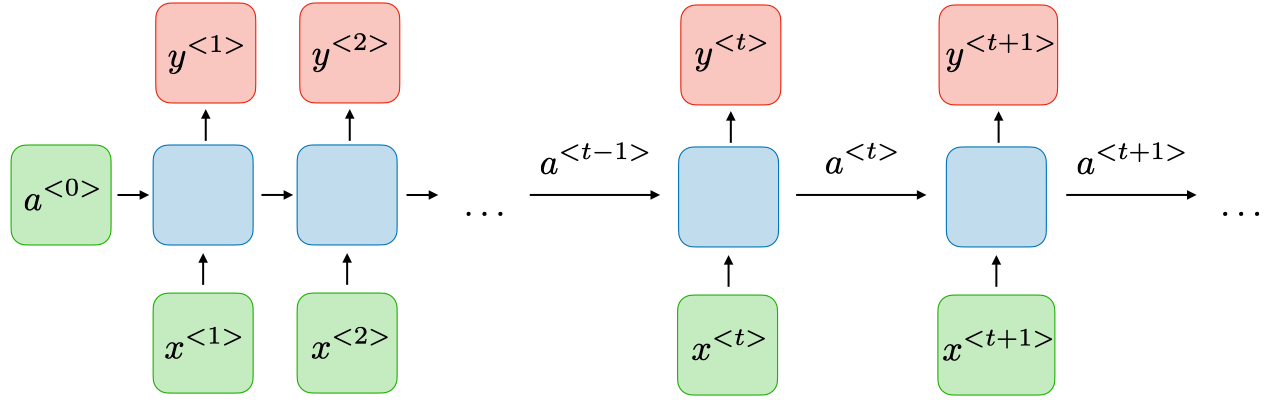
\includegraphics[width=0.49\textwidth]{Fig/1.png}
   \caption{Plot of Architecture of a traditional RNNRecurrent neural networks, also known as RNNs, a class of neural networks that allow previous outputs to be used as inputs while having hidden states.} \label{fig1}
\end{figure}

Recurrent Neural Networks (RNNs) are a class of neural networks specifically designed to handle sequential data. At the core of RNN architecture lies the unique feature of maintaining a form of memory that captures information about previous elements in the sequence. Unlike traditional neural networks, which assume independence between inputs, RNNs can process input data in a sequential manner, retaining state information from one step of the sequence to the next. This is achieved through loops within the network architecture, allowing information to persist.

One of the key strengths of RNNs is their ability to manage varying input lengths. In time series forecasting, such as cryptocurrency trading, where the input sequences can be of different durations, RNNs adaptively process this variable-length data, making them highly suitable for this domain~\cite{HochreiterSchmidhuber}. Furthermore, RNNs can not only process single data points (such as a day's closing price) but also sequences of data (such as prices over the past week), which is essential in understanding the temporal dynamics of financial markets.

\begin{figure}[htbp]
   \centering
   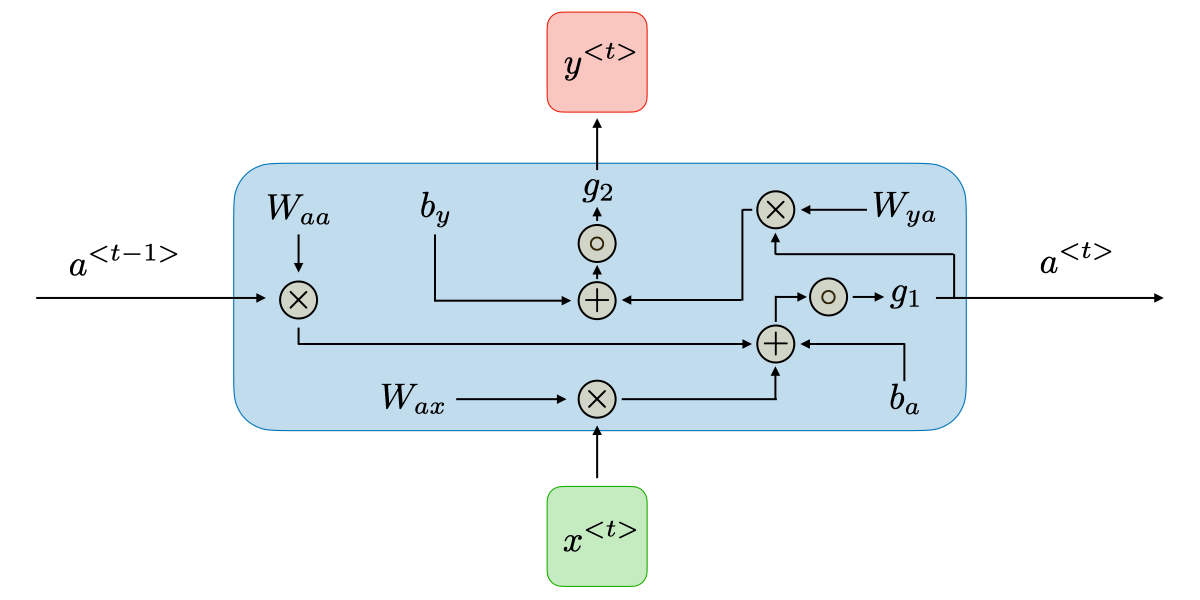
\includegraphics[width=0.49\textwidth]{Fig/2.png}
   \caption{Plot of how the information in time step $t-1$ influence time step $t$ in a traditional RNN model.} \label{fig2}
\end{figure}

However, traditional RNNs face challenges such as the vanishing gradient problem, which hinders the learning of long-range dependencies within the sequence data. This is particularly problematic in financial time series, where long-term trends and cycles are critical. To address this, variants of RNNs, like Long Short-Term Memory (LSTM) networks and Gated Recurrent Units (GRUs), have been developed~\cite{FuzzyInferenceLSTM}. These architectures incorporate mechanisms to control and maintain a balance between short-term input and long-term historical information, thus effectively capturing dependencies across different time scales.

\subsubsection{Long Short-Term Memory (LSTM) Networks}

Long Short-Term Memory (LSTM) networks, a significant advancement in the field of recurrent neural networks (RNNs), were introduced by Sepp Hochreiter and Jürgen Schmidhuber in 1997~\cite{FuzzyInferenceLSTM}. The primary motivation behind the development of LSTMs was to address the limitations of traditional RNNs, particularly their inability to learn long-term dependencies in sequence data. This inability, known as the vanishing gradient problem, arises because the gradients, which are used to update the network's weights, tend to either vanish or explode as they are propagated back through time in a deep network.

\begin{figure}[htbp]
   \centering
   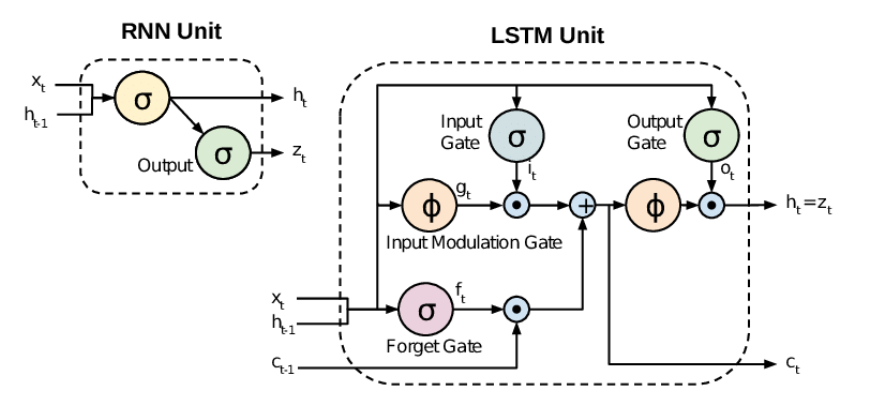
\includegraphics[width=0.49\textwidth]{Fig/3.png}
   \caption{Plot of a demo what the differences between RNN and lstm in handling input.} \label{fig3}
\end{figure}


LSTMs tackle this problem by incorporating a complex mechanism of gates, namely the input gate, forget gate, and output gate. These gates effectively regulate the flow of information into and out of the cell state, a central concept in LSTM architecture. The cell state acts as a kind of "memory" of the network, carrying relevant information throughout the sequence of data. The input gate controls how much new information is added to the cell state, the forget gate decides what information is discarded, and the output gate determines what information from the cell state should be used to generate the output at each timestep.

This architecture differs significantly from traditional RNNs and another variant, Gated Recurrent Units (GRUs). While GRUs also aim to solve the vanishing gradient problem, they do so with a simpler structure that combines the input and forget gates into a single "update gate" and merges the cell state and hidden state. In contrast, LSTMs maintain separate cell and hidden states, providing a more nuanced approach to information regulation. This allows LSTMs to capture longer and more complex temporal dependencies compared to RNNs and GRUs, albeit at the cost of increased computational complexity.

\begin{algorithm*}
   \caption{Long Short-Term Memory (LSTM) Pseudocode}
   \begin{algorithmic}[1] % The number tells where the line numbering should start
      \Procedure{LSTM}{input}
      \State Initialize cell state $c$ and hidden state $h$
      \State Initialize weight matrices $W_{xi}$, $W_{xf}$, $W_{xo}$, $W_{xc}$, $W_{hi}$, $W_{hf}$, $W_{ho}$, $W_{hc}$
      \State Initialize bias vectors $b_{i}$, $b_{f}$, $b_{o}$, $b_{c}$
      \For{each element $x_t$ in input}
      \State $i_t \gets \sigma(W_{xi} \cdot x_t + W_{hi} \cdot h_{t-1} + b_{i})$ \Comment{Input gate}
      \State $f_t \gets \sigma(W_{xf} \cdot x_t + W_{hf} \cdot h_{t-1} + b_{f})$ \Comment{Forget gate}
      \State $o_t \gets \sigma(W_{xo} \cdot x_t + W_{ho} \cdot h_{t-1} + b_{o})$ \Comment{Output gate}
      \State $\tilde{c}_t \gets \tanh(W_{xc} \cdot x_t + W_{hc} \cdot h_{t-1} + b_{c})$ \Comment{Candidate cell state}
      \State $c_t \gets f_t \ast c_{t-1} + i_t \ast \tilde{c}_t$ \Comment{Update cell state}
      \State $h_t \gets o_t \ast \tanh(c_t)$ \Comment{Update hidden state}
      \State $y_t \gets \text{softmax}(W_{hy} \cdot h_t + b_{y})$ \Comment{Compute output}
      \State Append $y_t$ to output sequence
      \EndFor
      \State \textbf{return} output sequence
      \EndProcedure
   \end{algorithmic}
\end{algorithm*}

\section{Experimentation} \label{sec:experimentation}

\subsection{Data Preprocessing}


\subsubsection{Data Acquisition}

The Binance API serves as a powerful interface that facilitates automated trading by granting programmatic access to Binance's market data and trading functionalities. In the realm of quantitative trading for cryptocurrencies, this API is an indispensable tool for acquiring real-time and historical market data, executing trades, and managing accounts.

Specifically, the utilization of the Binance Spot API within the provided code allows for the retrieval of K-line (candlestick) data for a specified cryptocurrency, such as Ethereum (ETH). K-line data is of paramount importance in financial analysis and trading strategy development, as it encapsulates critical market information over predefined time intervals. Each K-line, or candlestick, represents four vital data points within a given time frame: the opening price, the highest price, the lowest price, and the closing price. Additionally, it often includes trading volume data.

Within the provided script, functions like $get\_klines\_data$ facilitate the retrieval of this data from the Binance API. The script is meticulously designed to fetch ETH K-line data across various time scales (e.g., 1 minute, 1 hour), providing flexibility for the analysis of market trends across different time horizons. This acquired data forms the foundational basis for feature engineering, pattern recognition, and the development of predictive models within quantitative trading strategies. Consequently, traders can make well-informed decisions backed by comprehensive market insights.


\subsubsection{Data Augmentation and Price Normalization}

In the context of quantitative trading, data augmentation involves enriching the dataset with additional features derived from raw data. This process, often referred to as feature engineering, is crucial for capturing various aspects of market behavior and improving the predictive capability of trading models.

The following code showcases a comprehensive approach to augmenting cryptocurrency market data, focusing on various technical indicators and normalization techniques:

\begin{enumerate}
   \item \textbf{Technical Indicators}: The code computes several key technical indicators used in trading analysis, including:
         \begin{itemize}
            \item \textbf{Simple Moving Average (SMA) and Exponential Moving Average (EMA)}: These indicators smooth out price data over a specified period, highlighting the underlying trend by reducing short-term fluctuations.
            \item \textbf{Relative Strength Index (RSI)}: RSI measures the magnitude of recent price changes to evaluate overbought or oversold conditions.
            \item \textbf{Bollinger Bands}: This indicator provides a relative view of high and low prices, using a moving average and a standard deviation band.
            \item \textbf{Average True Range (ATR)}: ATR measures market volatility by decomposing the entire range of an asset price for that period.
            \item \textbf{On-Balance Volume (OBV)}: OBV uses volume flow to predict changes in stock price.
         \end{itemize}

   \item \textbf{Normalization of Price Data}: Price normalization is a critical step in preparing data for machine learning models. The script applies percentage change normalization to the price columns ('Open', 'High', 'Low', 'Close'). This technique transforms the price data into the rate of change, making the model less sensitive to absolute price levels and more responsive to relative price movement.

   \item \textbf{Standardization of Other Features}: For non-price features, the code uses standard scaling (z-score normalization). This process involves subtracting the mean and dividing by the standard deviation for each feature, ensuring that each feature contributes equally to the model's performance and improving the convergence speed during training.

   \item \textbf{Handling Missing Values}: The code fills any missing values using forward-fill (propagating the last observed non-null value to the next) and then removes any remaining rows with NaN values. This step maintains the consistency and integrity of the dataset, especially important with time-series data where chronological order and continuity are critical.

\end{enumerate}

After these methods, the data augmentation process transforms raw market data into a more analytically useful form. By incorporating technical indicators and applying normalization techniques, the dataset becomes better suited for training sophisticated machine learning models in quantitative trading. This enhanced dataset is crucial for capturing complex market dynamics and improving the predictive accuracy of trading algorithms.

\subsection{Experimentation Environment}

Our project's experimentation is conducted within a high-performance computing system, featuring the following specifications:

\begin{itemize}
   \item \textbf{RAM}: 256 GB
   \item \textbf{GPU}: NVIDIA GeForce RTX 3090
   \item \textbf{CPU}: Intel Xeon CPU E5-2696 v3
   \item \textbf{OS}: Ubuntu 22.04 LTS with kernel 6.2.0-37-generic
   \item \textbf{Programming Language}: Python 3.11.5
   \item \textbf{Deep Learning Framework}: PyTorch 2.1.0
\end{itemize}

This computing environment offers an exceptional balance of processing power and efficiency, making it well-suited for handling the demanding computational requirements of deep learning models in cryptocurrency trading. The Ubuntu operating system ensures stability and versatility, providing a reliable platform for various machine learning tasks. Additionally, with its substantial 256 GB of RAM, this system is capable of effortlessly managing large datasets and conducting complex calculations. Python 3.11.5 and PyTorch 2.1.0 are employed, with PyTorch's flexibility catering to the dynamic nature of financial data analysis and model experimentation.This environment is pivotal in facilitating efficient processing, analysis, and the development of robust and reliable trading strategies.


\begin{table*}[ht]

   \footnotesize
   \centering
   \begin{tabular}{lccccc}
      \hline
      Hyperparameter                  & Losses & Train Sharpe Ratios & Train Annualized Returns & Test Sharpe Ratios & Test Annualized Returns \\ \hline
      $conv\_2\_rnn\_1\_hidden\_50$   & 0.0025 & -0.891              & 0.046                    & -0.982             & -0.127                  \\
      $conv\_2\_rnn\_2\_hidden\_50$   & 0.0026 & -1.147              & 0.040                    & -1.244             & -0.103                  \\
      $conv\_2\_rnn\_2\_hidden\_100$  & 0.0025 & -0.927              & 0.044                    & -1.017             & -0.121                  \\
      $conv\_2\_rnn\_2\_hidden\_200$  & 0.0026 & -0.920              & 0.045                    & -1.013             & -0.124                  \\
      $conv\_2\_rnn\_2\_hidden\_400$  & 0.0027 & -1.464              & 0.032                    & -1.559             & -0.077                  \\
      $conv\_2\_rnn\_4\_hidden\_50$   & 0.0025 & -0.891              & 0.046                    & -0.982             & -0.127                  \\
      $conv\_2\_rnn\_8\_hidden\_50$   & 0.0025 & -0.891              & 0.046                    & -0.983             & -0.127                  \\
      $conv\_3\_rnn\_1\_hidden\_50$   & 0.0025 & -0.890              & 0.046                    & -0.982             & -0.127                  \\
      $conv\_3\_rnn\_2\_hidden\_50$   & 0.0025 & -0.891              & 0.046                    & -0.982             & -0.127                  \\
      $conv\_3\_rnn\_2\_hidden\_100$  & 0.0025 & -0.895              & 0.046                    & -0.985             & -0.127                  \\
      $conv\_3\_rnn\_2\_hidden\_200$  & 0.0025 & -0.899              & 0.045                    & -0.990             & -0.125                  \\
      $conv\_3\_rnn\_2\_hidden\_400$  & 0.0025 & -0.903              & 0.047                    & -0.999             & -0.134                  \\
      $conv\_3\_rnn\_4\_hidden\_50$   & 0.0025 & -0.891              & 0.046                    & -0.982             & -0.127                  \\
      $conv\_3\_rnn\_8\_hidden\_50$   & 0.0025 & -0.891              & 0.046                    & -0.983             & -0.127                  \\
      $conv\_4\_rnn\_1\_hidden\_50$   & 0.0025 & -0.891              & 0.046                    & -0.982             & -0.127                  \\
      $conv\_4\_rnn\_2\_hidden\_50$   & 0.0025 & -0.891              & 0.046                    & -0.982             & -0.127                  \\
      $conv\_4\_rnn\_2\_hidden\_100$  & 0.0025 & -0.891              & 0.046                    & -0.982             & -0.127                  \\
      $conv\_4\_rnn\_2\_hidden\_200$  & 0.0025 & -0.893              & 0.046                    & -0.985             & -0.127                  \\
      $conv\_4\_rnn\_2\_hidden\_400$  & 0.0025 & -0.901              & 0.045                    & -0.991             & -0.123                  \\
      $conv\_4\_rnn\_4\_hidden\_50$   & 0.0025 & -0.891              & 0.046                    & -0.982             & -0.127                  \\
      $conv\_4\_rnn\_8\_hidden\_50$   & 0.0025 & -0.891              & 0.046                    & -0.982             & -0.127                  \\
      $conv\_5\_lstm\_2\_hidden\_200$ & 0.0025 & -0.891              & 0.046                    & -0.982             & -0.127                  \\
      $conv\_5\_rnn\_1\_hidden\_50$   & 0.0025 & -0.891              & 0.046                    & -0.982             & -0.127                  \\
      $conv\_5\_rnn\_2\_hidden\_50$   & 0.0025 & -0.891              & 0.046                    & -0.982             & -0.127                  \\
      $conv\_5\_rnn\_2\_hidden\_100$  & 0.0025 & -0.891              & 0.046                    & -0.982             & -0.127                  \\
      $conv\_5\_rnn\_2\_hidden\_200$  & 0.0025 & -0.891              & 0.046                    & -0.982             & -0.127                  \\
      $conv\_5\_rnn\_2\_hidden\_400$  & 0.0025 & -0.895              & 0.045                    & -0.986             & -0.125                  \\
      $conv\_5\_rnn\_4\_hidden\_50$   & 0.0025 & -0.891              & 0.046                    & -0.982             & -0.127                  \\
      $conv\_5\_rnn\_8\_hidden\_50$   & 0.0025 & -0.891              & 0.046                    & -0.982             & -0.127                  \\
   \end{tabular}
   \caption{Metrics of Models with Different Complexities. Note, all the results performed poorly on such a long time series (From 01/01/2017 to 31/12/2022 with time scale 1 day). This results suggest that the RNN and LSTM model are not able to learn the patterns in such a long data.}
   \label{tab:performance_metrics_transposed}
\end{table*}

\subsection{Experimental Parameters and Model Hyperparameter Selection}

Our experimental framework has been meticulously designed to encompass a wide range of parameters and hyperparameters, which are crucial for evaluating the effectiveness of various trading strategies under diverse scenarios. At the core of our experimentation, we employ a diverse array of model architectures, specifically tailored to meet the unique requirements of financial time series data.

We explore multiple configurations of convolutional and recurrent neural network layers to understand their impact on the model's predictive capabilities. These configurations range from simpler setups, such as two-layer convolutional networks, to more complex structures involving up to five layers. Similarly, our recurrent neural network configurations vary, including different combinations of hidden layer sizes and numbers of layers. This diversity in model architecture allows us to navigate the trade-off between computational efficiency and the depth of learning required for accurate market predictions.

The training process is enhanced with sophisticated data handling and optimization techniques. We implement both a standard Trainer class and a more advanced GroupedTrainer. The latter divides the dataset into manageable groups for more efficient training, a particularly beneficial approach for handling the large datasets common in financial applications. Our choice of loss functions is based on the nature of the problem, with binary cross-entropy for two-class problems, cross-entropy for multi-class scenarios, and mean squared error for regression tasks. This careful selection ensures that the loss computation aligns with the specific objectives of each model. Additionally, we utilize the Adam optimizer, known for its adaptability and effectiveness, especially with sparse gradients. A step-based learning rate scheduler is employed to periodically reduce the learning rate, fine-tuning the models as training progresses. This methodical optimization approach aids in achieving a balance between quick convergence and avoiding local minima.

To evaluate model performance, we employ a combination of traditional machine learning metrics and financial performance indicators. Metrics like the Sharpe ratio and annualized returns are included to provide a clear picture of the risk-adjusted returns of our trading strategies, a critical aspect in financial modeling. Our training regimen extends over 7200 epochs with evaluations conducted at regular intervals, ensuring thorough exploration of the learning capacity of each model configuration.

Furthermore, our framework is designed to be flexible in handling different data formats, with functions to process both numpy arrays and pandas DataFrames. This flexibility is crucial for seamless integration with varied data sources commonly encountered in financial modeling. The computational aspect is efficiently managed by deploying models on the most suitable hardware available, whether it be CPU or GPU, thereby optimizing resource utilization and ensuring expedient model training and evaluation.

\section{Results} \label{sec:results}

\subsection{Challenges Posed by Extended Time-Series in Training}

The experimental results obtained from our comprehensive models, designed to predict financial market trends using daily data spanning from 2012 to 2022, reveal significant challenges in model performance, as indicated by the negative Sharpe ratios and suboptimal annualized returns. This observation prompts a critical analysis of the potential issues arising from training models on extended time-series data. One of the primary challenges in such scenarios is the inherent complexity and variability of financial markets over long periods. Financial markets are influenced by a multitude of factors, including economic changes, political events, and market sentiment, all of which evolve over time. The data spanning a decade encapsulates multiple market cycles, including bull and bear phases, recessions, and recoveries. As a result, the model is required to generalize across highly diverse market conditions, a task that proves challenging for even sophisticated models like RNNs and LSTMs.

Another issue stems from the nature of traditional time-series models, which are typically adept at capturing short- to medium-term dependencies but may struggle with long-term historical data. This limitation is evident in our models’ inability to effectively leverage the full depth of information present in a decade-long dataset. The problem is further compounded by the fact that financial time-series data is often non-stationary, meaning its statistical properties, such as mean and variance, change over time. This non-stationarity makes it difficult for models to learn stable and generalizable patterns, particularly when the training data encompasses extended periods with varied market dynamics. Moreover, the sheer volume of data associated with long-term time series introduces additional computational challenges. Training deep learning models on such extensive datasets demands significant computational resources and time, often leading to practical constraints in iterative model tuning and experimentation. There is also a risk of overfitting, where the model learns specific patterns or noise present in the training data, which do not generalize well to unseen market conditions.

\textbf{Note:} In the context of our experiments, the term $'hyperparameter'$ specifically pertains to the architecture and configuration of the convolutional and recurrent neural network (RNN) layers used in our models. To illustrate this, consider the naming convention $'conv\_2\_rnn\_2\_hidden\_100,'$ where each component signifies a particular configuration:

\begin{itemize}
   \item \textbf{$'conv\_2'$} refers to the configuration of the convolutional layers and is defined in the $'conv\_configs'$ list. In this example, '2' indicates the use of two convolutional layers with specific configurations provided in the corresponding index of the $'conv\_configs'$ list. For instance, [(32, 3, 1), (64, 3, 1)] signifies two convolutional layers, with the first layer having 32 filters, a kernel size of 3, and a stride of 1, while the second layer has 64 filters, also with a kernel size of 3 and a stride of 1.

   \item \textbf{$'rnn\_2'$} and $'hidden\_100'$ pertain to the configuration of the recurrent neural network (RNN) layers. $'rnn\_2'$ indicates that the model contains two RNN layers, while $'hidden\_100'$ signifies that each of these layers has 100 neurons or hidden units. The number of RNN layers and the number of neurons in each layer are critical factors in determining the model's capacity to learn and capture patterns in the data, particularly in time-series analysis where temporal dependencies are paramount.
\end{itemize}

\begin{table}
   \footnotesize
   \centering
   \begin{tabular}{lccc}
      \hline
      Dataset len & Losses & Train Accuracy & Test Accuracy \\ \hline
      $100$       & 0.7    & 0.56           & 0.64          \\
      $200$       & 0.7    & 0.51           & 0.57          \\
      $400$       & 0.72   & 0.45           & 0.59          \\
      $800$       & 0.69   & 0.51           & 0.56          \\
      $1600$      & 0.69   & 0.5            & 0.36          \\
   \end{tabular}
   \caption{Metrics of Models with Different dataset length. Note, the value in $dataset length$ means the number of dataset, instead the time scales of all dataset.}
   \label{tab:performance_metrics_transposed}
\end{table}

\subsection{Limitations of RNN and LSTM in Handling Extended Time-Series}

Our recent results, obtained through a modified approach where we transformed our task into a classification problem, have unveiled a critical limitation inherent in Recurrent Neural Networks (RNNs) and Long Short-Term Memory (LSTM) networks when dealing with extended time-series data. The performance metrics, particularly when observed across varying lengths of the dataset, reveal a significant challenge in model efficacy as the length of the time-series increases.

Initially, for shorter time-series lengths (e.g., 100 and 200 data points), the models exhibited relatively higher accuracy. However, with an increase in the length of the time-series data (400, 800, and especially 1600 data points), a noticeable decline in both training and testing accuracy became evident. This pattern suggests that RNNs and LSTMs, despite being designed for sequential data, encounter difficulties in effectively capturing and utilizing information from lengthy time-series. This issue is often attributed to the vanishing gradient problem, where gradients used in training the network diminish or explode as they propagate back through extended sequences during training, impeding the model's ability to learn dependencies over prolonged periods.

Furthermore, financial time-series data often encompass complex and evolving market dynamics that are challenging to encapsulate in a model trained on lengthy historical sequences. These dynamics can include non-stationary behaviors, where statistical properties of the data, such as mean and variance, change over time. As the length of the time-series increases, the model's ability to generalize and adapt to such changes becomes increasingly challenging.

Another consideration is the practicality of training deep learning models on extensive datasets. Training on longer sequences demands substantial computational resources and time. Often, the increase in data length does not proportionally translate to an increase in informative content for the model. This scenario can lead to inefficiencies and potential overfitting, where the model might learn noise or irrelevant patterns present in the extended data sequences.

\section{Summary and Conclusion} \label{sec:summary}

Our extensive experimentation with RNNs and LSTMs in predicting financial market trends using a decade's worth of daily data has brought to light several critical insights and challenges. The models, while designed to handle sequential data, revealed significant limitations when applied to extended time-series, as evidenced by the declining accuracy with increasing dataset lengths. This trend suggests a fundamental issue in these models' ability to process and learn from long-term dependencies, a critical requirement in financial time-series analysis. One of the inherent issues is the vanishing gradient problem, which becomes more pronounced with longer sequences, leading to difficulties in learning across such extensive periods. Moreover, the complexity and non-stationary nature of financial markets add to the challenge, as these models struggle to generalize across the various market conditions encapsulated in a lengthy dataset.

In addition to these challenges, our experiments highlighted the importance of data representation and feature selection in modeling financial markets. We observed that using closing prices and computing returns by dividing the subsequent day's price by the previous day's price (minus one) could yield more informative features than raw prices. This approach to feature engineering aligns with the underlying financial theory and provides a more standardized and relative measure of market movements. Furthermore, incorporating traditional financial analysis techniques as inputs to the neural networks could enhance model performance. This integration suggests that blending traditional financial wisdom with advanced machine learning techniques can be a more effective strategy than relying solely on complex models.

Another key takeaway from our experiments is the realization that complexity in model architecture does not necessarily translate to better performance, especially in a market characterized by high noise levels like the stock market. There is a delicate balance between model complexity and the risk of overfitting, particularly in a domain where the signal-to-noise ratio is inherently low. Neural networks, while powerful, may also learn and amplify the noise present in the data, making long-term predictions challenging and less reliable.

Looking forward, considering the dynamic and real-time nature of stock markets, adopting online learning approaches could be a more effective strategy. Online learning, where the model continuously updates itself with new data, can potentially adapt more swiftly to market changes and evolving trends. This approach could address some of the challenges posed by the non-stationary nature of financial data and improve the model's responsiveness to recent market dynamics.

In conclusion, our comprehensive analysis underscores the need for a nuanced approach in applying deep learning models to financial time-series prediction. The challenges posed by extended time-series data necessitate a careful consideration of model architecture, feature engineering, and learning strategies. The integration of traditional financial analysis with machine learning, careful balancing of model complexity, and exploration of online learning methodologies emerge as promising directions for future research in this domain.


   % we~\cite{Authors14b} we.1
   {
      \small
      \bibliographystyle{ieeenat_fullname}
      \bibliography{main}
   }





% WARNING: do not forget to delete the supplementary pages from your submission 
% \input{sec/X_suppl}

\end{document}
